\chapter{(Future) Methodology}
\label{cha:methodology}

\section{Data analysis}
\label{sec:method}

\begin{figure*}[h]
  \label{fig:flowchart}
  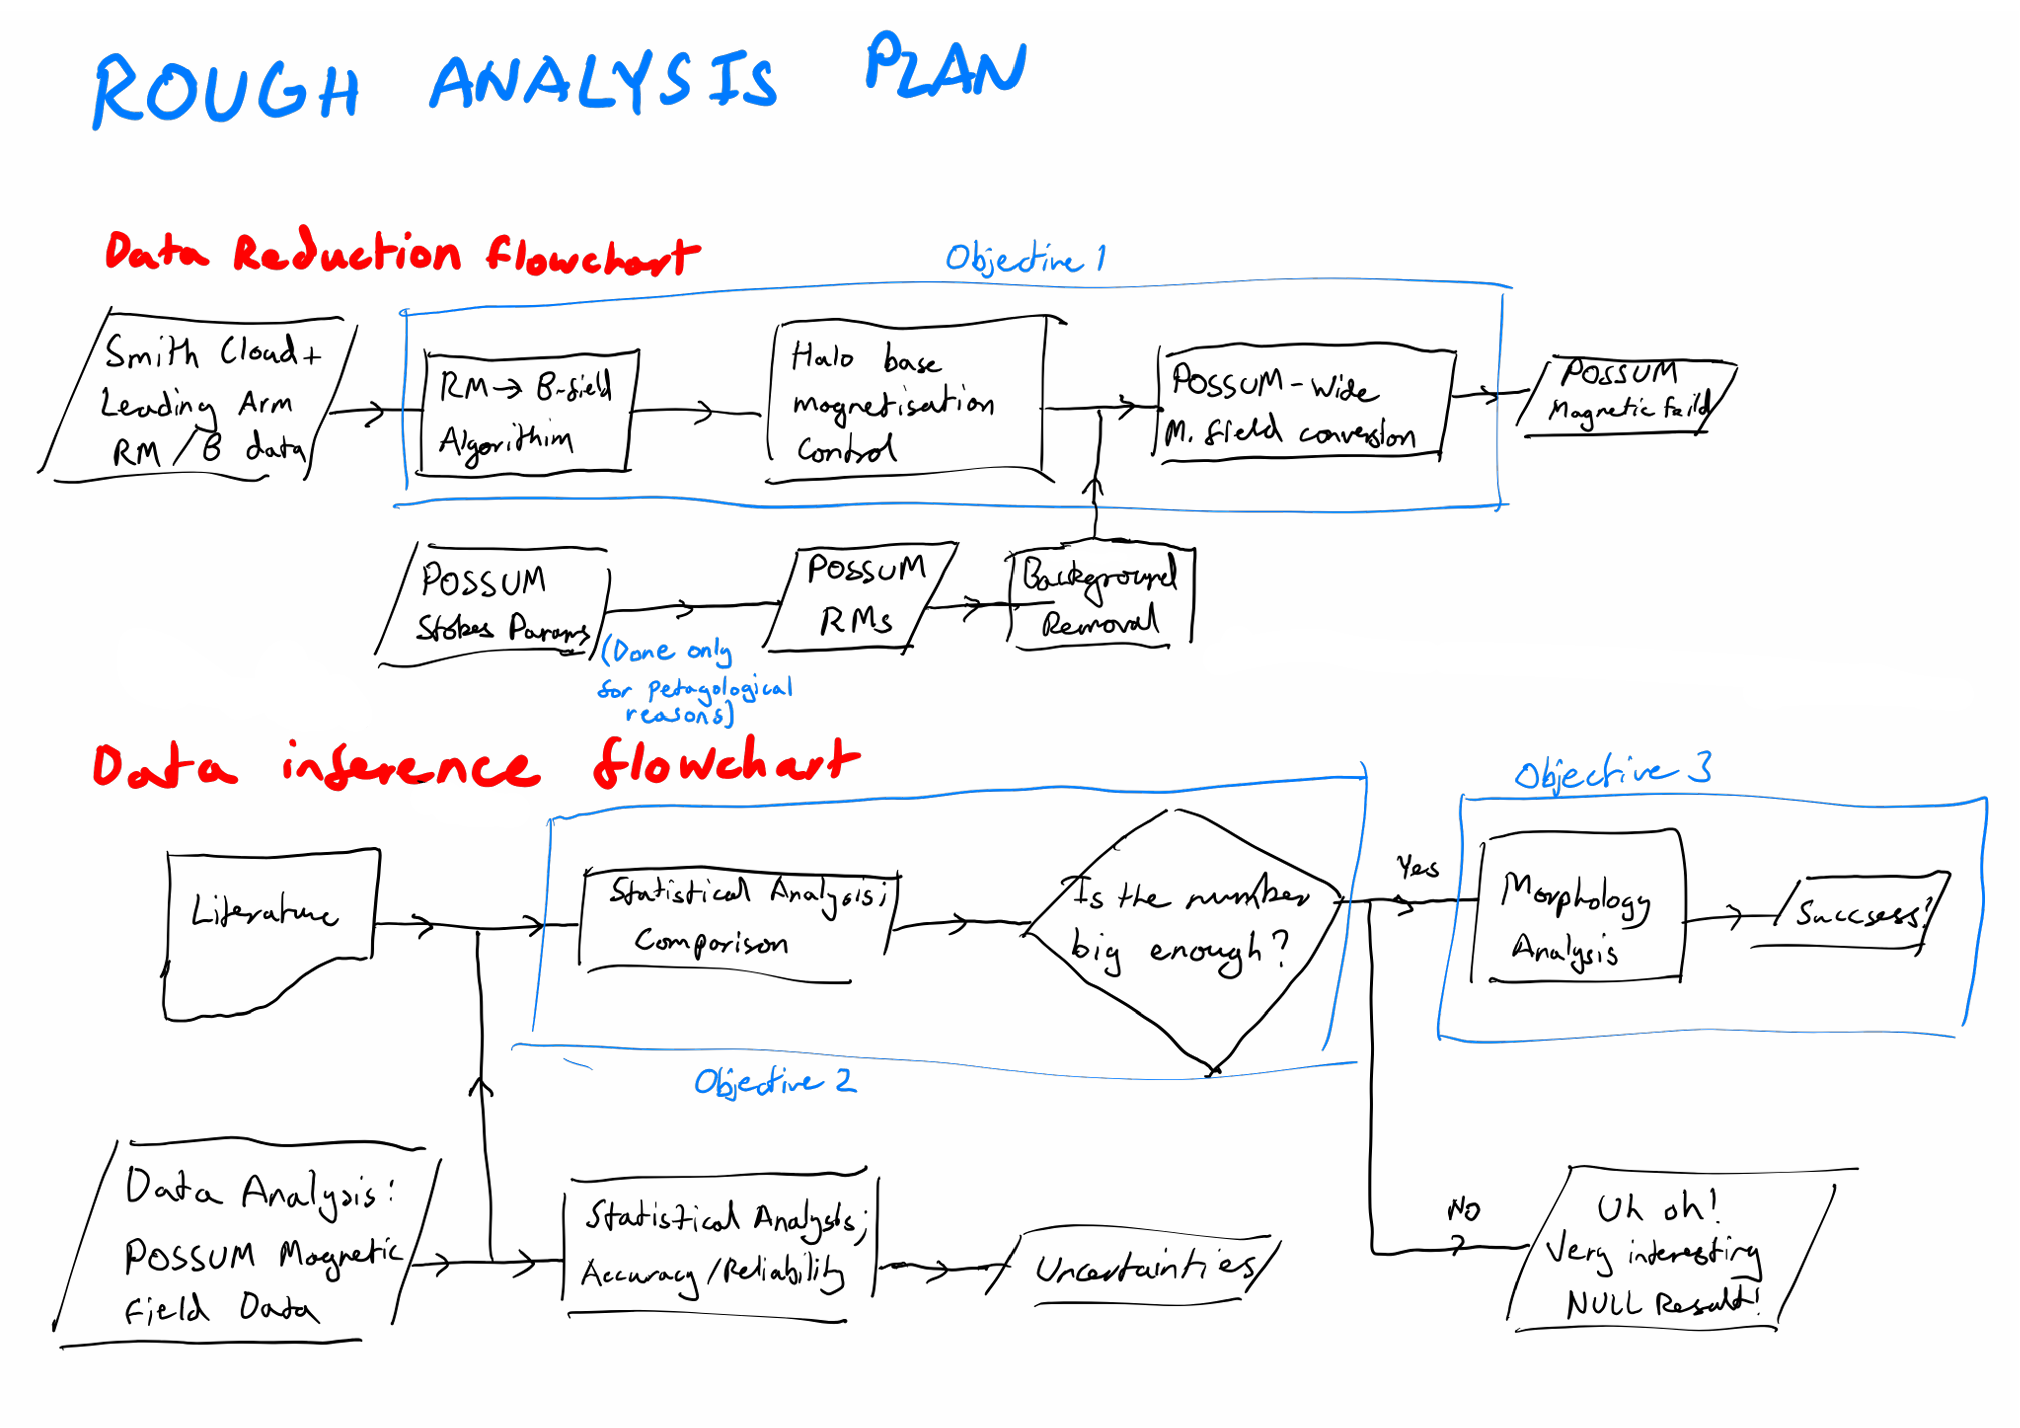
\includegraphics[width=\columnwidth]{figs/flowchart.png}
  \caption{A rough flowchart of the data analysis method. A neater version of this flowchart will appear in future iterations of the report as a visual representation of the methodology.}
\end{figure*}

Figure~\ref{fig:flowchart} represents the rough outline of the pipeline of data analysis as per the three objectives listed in \ref{sec:objectives}.

The first point of data reduction is to convert the raw POSSUM data, i.e. stokes parameters in the field, to RMs. A component of research, revision, and programming will be dedicated to doing this. POSSUM as a survey has already condensed the stokes parameters into RMs \cite{ID1}. The purpose of doing it again is purely for pedagogical reasons - so that a better understanding about the nature of RMs is achieved. Purposefully, this part of the data reduction will only appear in perhaps a few sentences in the mid-term and final report, discussing how the POSSUM data was obtained.

SC data will be obtained from a secondary source outside of POSSUM \cite{ID18, ID26, ID28}. The purpose of this data is to act as a testing set. Since past research has already determined the magnetic field strengths in HVCs in those regions \cite{ID26}. It is important that this data be used to confirm that the algorithm developed is working correctly.

After the program is developed to convert RMs into magnetic fields, data from the non-active components of the halo itself are then fed through the same algorithm. This will act as a control variable, providing a measure of base magnetisation for the Galactic Halo as well as pointing to a default ionisation state of the halo.

The halo control test will also help in the removal of background and foreground sources of Faraday rotation \footnote{Background removal will also be performed using the annulus method}. The light used to measure polarisation, comes from extragalactic synchrotron radiation, and is initially unpolarised. However, this radiation will have to travel a far distance before reaching us, at which point it can polarise from ionised gas in the Universe. HVCs will also be ionised. this is where H-alpha and foreground observations are used, as they provide information of the emission measure of the HVCs.

All these sources of interference can make it extremely difficult to determine the actual RMs. A background control run and analysis of the HVC can prevent this issue. Combating RM interference is an active part of the process in radio astronomy, with research that aims to tackle this problem \cite{ID21}. With a larger data set, however, there is more reliability simply because there is more resistance to outliers. In previous examples, HVCs in the can be obscured, which is a way HVCs in the halo can also experience faulty RMs \cite{ID2, ID36}.

Techniques for background removal include convolutional blurring, binned averages, median filtering, and signal whitening/bandpassing \cite{ID38, ID39, ID40}. Tools which will be investigated in literature while completing the implementation of objective 1.

Once all these processes are done, the algorithm should be fully capable of a simple pass-over across all HVCs in the entire southern sky. This step is the easiest, as it only involves repeatedly running an already completed script on several objects. After the program is developed, applied across all detected HVCs in the field, and the data is catalogued, the next step is to infer information from this data.

Most of the statistical analysis tools will be basic, as objective 2 simply requires a rough estimate of the magnetic field strengths. Uncertainties will naturally arise from the program's mathematical evaluations. The K-S test will be used to compare magnetic field distributions to theoretical cases and example cases like the SC. Simple averages, box plots, and other single-set analysis tools will be used to establish a characterisation of the sample. It is expected, however, that HVCs that are at a higher Galactic latitude will be more resolute as there is less contamination by dust radio emission from the disk. This should be accounted for in the analysis of uncertainties.

Once these tests have been performed, it will be possible to assess if the results align with the initial alternative hypothesis. From there, either a tertiary objective is completed (if there is time), or further research is recommended in the conclusion of the report.

\section{Timeline of honours project}
\label{sec:timeline}

\begin{table*}[ht]
  \centering
  \input table/timeline.tex
  \caption{A planned timeline of events.}
  \label{tab:timeline}
\end{table*}

Table~\ref{tab:timeline} displays a rough timeline of both honours program milestones and self-assigned objectives.

As a general summary, the first half of the first semester will be focused on initialising the project, starting the process of research, and planning. The second half will focus on primarily completing objective 1, in which 14 weeks sounds like a realistic timeframe. The midterm report will be worked on as the tasks of objective 1 approach completion, with all the new research discovered over those months being compiled into the incomplete skeleton of the report.

Objective 2 will require less time, and hence only will take the former half of the second semester. The latter half of the semester is dedicated to drafting and finalising the report and its results. After the second semester exams, there will be a bit of time to clean up the project's code for future use, debriefing on the year, and if the research is of enough value, potentially publishing the report.

I do not actually know, according to the honours guidelines, if I am allowed to submit theses for formal publishing after the grading and reviewing of the report internally.

There will inevitably be disruptions, to account for these, several contingency measures are employed:
\begin{enumerate}
\item Starting work on tasks 1-2 weeks before their allocated time
\item Spending a portion of the 20 hrs/week on non-focused tasks (i.e. reading for 3 hrs while working on objective 1)
\item Slightly overestimating the time it takes to complete each aspect of the project, to allow room for slow progress
\item Using a flowchart model of progression, so if one aspect of the project cannot be completed, only future contingencies are hindered
\item Regular and premature testing of programs
\end{enumerate}

%%% Local Variables: 
%%% mode: latex
%%% TeX-master: "paper"
%%% End: 
